%%%%%%%%%%%%%%%%%%%%%%%%%
% Dokumentinformationen %
%%%%%%%%%%%%%%%%%%%%%%%%%
\newcommand{\titleinfo}{Computertechnik 2 - Formelsammlung}
\newcommand{\authorinfo}{J.Rast}
\newcommand{\versioninfo}{$Revision: 991$}

\include{header/header}

%listing setting for asm code
\lstset{
	tabsize=2,
	rulecolor=,
	language=[Motorola68k]Assembler,
	basicstyle=\footnotesize\sffamily,
	frame=single,
	keywordstyle=\color[rgb]{0,0,1},
	commentstyle=\color[rgb]{0.133,0.545,0.133},
	stringstyle=\color[rgb]{0.627,0.126,0.941},
}



\begin{document}
\tableofcontents
\newpage

\section{Adressraum}
\begin{multicols}{2}
\begin{itemize}
  \item Bussystem: Verbindet die Komponenten
  	\begin{itemize}
  		\item CPU: Control Unit, Processing Unit
  			\begin{itemize}
  				\item Init Phase: CPU-Startup
  				\item Infinite Loop: "`fetch-execute"'-Cycle
			\end{itemize}
  		\item Memory: Programm, Daten
  		\item I/O: Inptut/Output
	\end{itemize}
  \item Komponenten eines Prozessor-Bussystem:
  	\begin{itemize}
  		\item Adress Bus: Uni-Direktional, bestimmt maximal adressierbarer Speicher
  		\item Data Bus: Bi-Direktional, überträgt Daten zwischen CPU und Memory
  		\item Control Bus: Überträgt Timing- und andere Steuer-Signale von der CPU an die I/O-Geräte
	\end{itemize}
\end{itemize}
\end{multicols}

\subsection{Stack}
Der Stack wächst immer von der höchsten Adresse zur tiefsten Adresse hin, der Stackpointer zeigt immer auf den obersten Eintrag im Stack (Top of Stack \textbf{ToS}).
Der Stack ist ein typischer \textbf{last-in first-out (LIFO)} Speicher. \\
Der Stack Pointer muss immer eine gerade Adresse halten. \\
\begin{tabular}{lll|l}
	\textbf{Push}	& move.w	& source, -(SP)			& siehe auch \textbf{movem}: push/pull list of registers \\
	\textbf{Pull}	& move.w	& (SP)+, destination	& movem.l \quad a1-a4/a6/d0-d3, -(a7)
\end{tabular}


\section{Subroutines}
Subroutinen stellen das gleiche dar wie Funktionsaufrufe in höheren Sprachen. Somit kann der gleiche Code mehrmals wiederverwendet werden.
\begin{itemize}
  \item Subroutine Aufruf: Inhalt von PC in den Stack, Sprung (jsr/bsr) in die Subroutine
  \item Subroutine Rückkehr: Inhalt vom Stack zurück in den PC.
\end{itemize}
\textbf{Achtung:} Eine Subroutine sollte nicht versuchen den "`Return-Pointer"' zu verändern. Dies führt zu Problemen wenn die Subroutine anders aufgerufen wird.

Normalerweise wird das Condition Code Register (CCR) durch die Subroutine beeinflusst. Möchte man das nicht kann das CCR auf dem Stack abgelegt werden und am Schluss wieder hergestellt werden: \\
\begin{lstlisting}
	  BSR GET_DATA
	GET_DATA: 
	  MOVE.W CCR,-(A7)  *CCR auf den Stack legen
	  RTR CCR           *zurueckschreiben und Subroutine verlassen
\end{lstlisting}


\section{Programm Strukturen}
\begin{tabular}{ll}
	\hline
	\textbf{if L then S} & \textbf{if L then S1 else S2} \\
  	\raisebox{0.55cm}{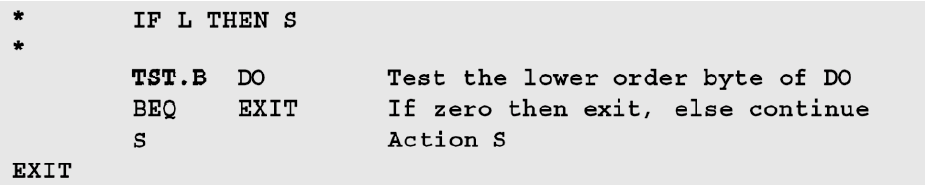
\includegraphics[width=9cm]{images/IfThen.PNG}} & 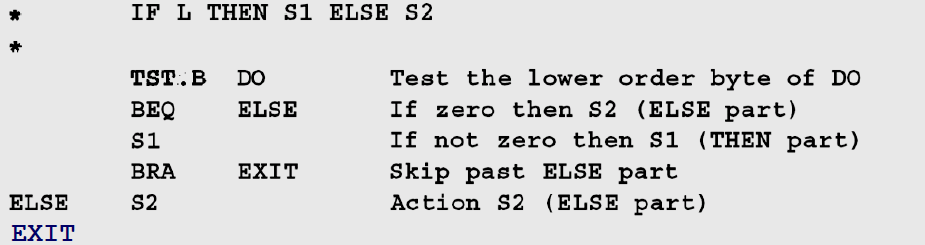
\includegraphics[width=9cm]{images/IfThenElse.PNG} \\
	\hline
	\textbf{for I=n1 to n2 do} & \textbf{while L do S} \\
  	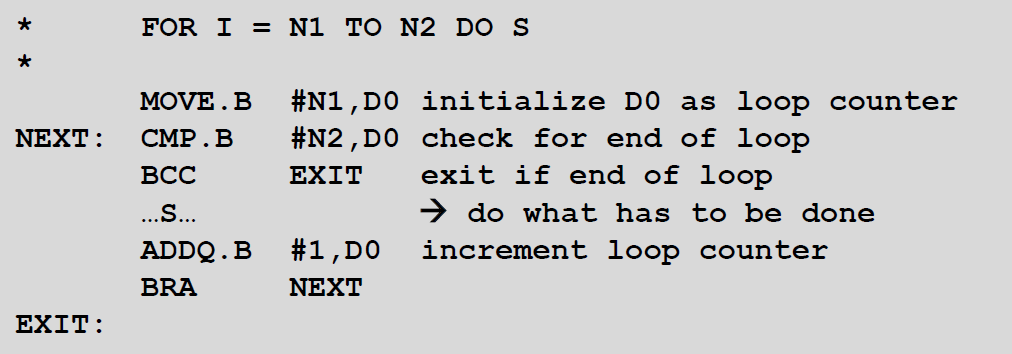
\includegraphics[width=9cm]{images/For.PNG} & \raisebox{0.9cm}{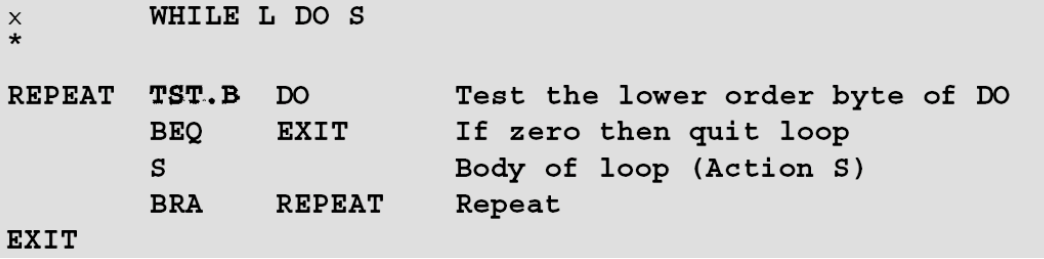
\includegraphics[width=9cm]{images/While.PNG}} \\
	\hline
	\textbf{case I of I1:S1, I2:S2 ,\ldots , default:Sd} & \textbf{repeat S until L} \\
  	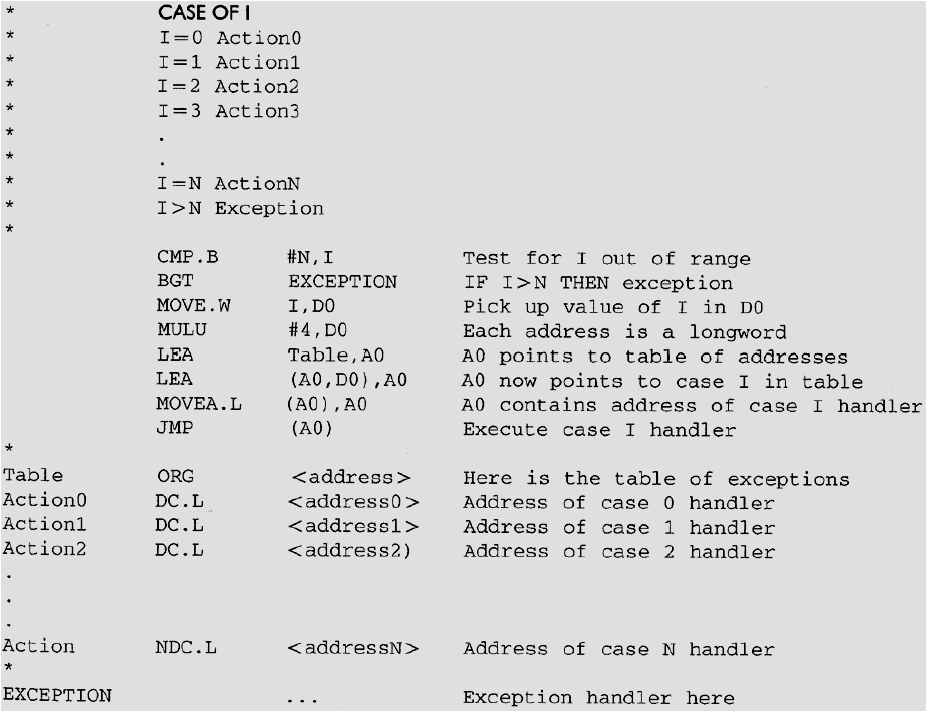
\includegraphics[width=9cm]{images/Case.PNG} & \raisebox{4.9cm}{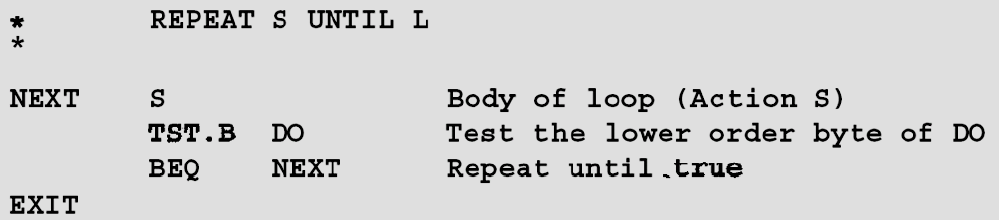
\includegraphics[width=9cm]{images/Repeat.PNG}} \\
	\hline
\end{tabular}

\section{Pseudocode (PDL)}
Pseudocode oder PDL (program developement language) bietet die möglichkeit Assembler Programme strukturierter zu erstellen in dem man PDL als persönliche Hochsprache verwendet.
Die PDL lässt sich nach belieben an die eigenen Bedürfnisse anpassen.
\section{Assembler und C}
\subsection{Prinzipien des Datenaustausch}
\begin{itemize}
  \item Wenn kein Informationsaustausch notwendig ist:
  	\begin{itemize}
  		\item Kein Datenaustausch zwischen Aufrufer und Subroutine
  		\item Alle lokal modifizierten Register sollten erhalten bleiben
	\end{itemize}
  \item Wenn Informationsaustausch notwendig ist:
  	\begin{itemize}
  		\item Klares Konzept zur Übergabe der Daten muss festgelegt werden
  		\item Alle lokal modifizierten Register sollten erhalten bleiben
	\end{itemize}
\end{itemize}


\subsubsection{Datenaustausch via Register}
\begin{itemize}
  \item Aufrufer legt Parameter in die gemeinsamen Register
  \item Subroutine holt sich die Parameter von den Register
  \item Resultate werden wider in die Register abgelegt
\end{itemize}
\begin{tabular}{p{0.35\textwidth}|l}
	\textbf{Vorteile} 	& \textbf{Nachteile} \\
	\hline
	schnell				& Anzahl Parameter limitiert \\
	kleiner Overhead	& Parameter und Register müssen klar definiert werden \\
						& nicht ablaufinvariant \\ 
						& parallele Interupts sind gefährlich
\end{tabular}


\subsubsection{Datenaustausch via Register-Windowing}
\begin{itemize}
  \item Aufrufer legt Parameter in sein output register-window
  \item Subroutine holt sich die Parameter von seinem input register-window
  \item Resultate werden in das input register-window abgelegt
\end{itemize}
\begin{tabular}{p{0.35\textwidth}|l}
	\textbf{Vorteile} 	& \textbf{Nachteile} \\
	\hline
	schnell				& Anzahl Parameter limitiert auf die grösse des register window \\
	kleiner Overhead	& Parameter und Register müssen klar definiert werden \\
						& Level der Subroutine Aufrufe ist beschränkt (bei Rekursion) \\
						& eventuell nicht ablaufinvariant \\ 
						& parallele Interupts sind gefährlich \\
						& Register-Windowing selten unterstützt
\end{tabular}


\subsubsection{Datenaustausch via globalen Speicher}
\begin{itemize}
  \item Aufrufer legt Parameter in den globalen Speicher
  \item Subroutine holt Parameter vom globalen Speicher
  \item Resultate werden in den globalen Speicher gelegt
\end{itemize}
\begin{tabular}{p{0.35\textwidth}|l}
	\textbf{Vorteile} 	& \textbf{Nachteile} \\
	\hline
	virtuell unlimitierte Anzahl Parameter	& Parameterstruktur muss klar definiert werden \\
											& Overhead durch schreiben/lesen der Parameter \\
											& globale Variablen sind gefährlich \\
											& nicht ablaufinvariant
\end{tabular}


\subsubsection{Datenaustausch via Stack}
\begin{itemize}
  \item Aufrufer und Subroutine legen/holen sich die Parameter vom Stack
  \item Aufrufer und Subroutine müssen die Reihenfolge und das Format der Parameter einhalten
  \item \textbf{Achtung:} Alle Parameter müssen wieder vom Stack entfernt werden!
\end{itemize}
\begin{tabular}{p{0.35\textwidth}|l}
	\textbf{Vorteile} 	& \textbf{Nachteile} \\
	\hline
	virtuell unlimitierte Anzahl Parameter	& eventuell schwieriger zum verstehen \\
	ablaufinvariant, Rekursion möglich 		& \\
	klar und strukturiert					&
\end{tabular}


\subsection{Mechanismen für die Parameterübergabe}
\begin{itemize}
  \item \textbf{by Value:}
  	\begin{itemize}
  		\item Die Subroutine erhält eine Kopie der Originaldaten
  		\item Modifikation der Daten ändert die Originaldaten nicht
	\end{itemize}
  \item \textbf{by Reference:}
  	\begin{itemize}
  		\item Die Subroutine erhält ein Pointer auf die Daten
  		\item Die Daten werden nicht kopiert, änderungen der Daten in der Subroutine bleiben erhalten
	\end{itemize}
  \item \textbf{Return Values}
  	\begin{itemize}
  		\item via vorbestimmtes Datenregister
  		\item \textbf{MC68'000:} Typischerweise wird das Datenregister D0 für den Rückgabewert verwendet.
	\end{itemize}
\end{itemize}


\subsection{Lokale Variablen und Stack Frames}
Eine Subroutine braucht eventuell einen bestimmten Speicher um lokale Variablen zu speichern. Für diesen Speicher gibt es zwei Möglichkeiten: \\
\textbf{Statische Allokation}
\begin{itemize}
  \item Fixer Adressraum für die lokalen Variablen
  \item Funktioniert nur wenn die Subroutine nicht ablaufinvariant und nicht rekursiv ist
\end{itemize}
\textbf{Dynamische Allokation}
\begin{itemize}
  \item Variablen auf den Stack ablegen
  \item Mit den Instruktionen \verb+LINK+ und \verb+UNLK+ kann ein Stack Frame, eine temporäre Region auf dem Stack angelegt werden
  \item Das Stack Frame wird für jeden Aufruf der Subroutine neu angelegt, somit ist Rekursion möglich
  \item Das Stack Frame ist über einen \textbf{Frame Pointer} erreichbar
\end{itemize}


\subsubsection{LINK und UNLK Instruktion}
\begin{tabular}{l|l}
	\verb+LINK+											& \verb+UNLK+ \\
	Stack Frame erstellen								& Stack Frame löschen \\
	\hline
	\verb+LINK A6,#-16+									& \verb+UNLK A6+ \\
	Stack Pointer um 4 verkleinern						& Inhalt von A6 in den Stack Pointer laden \\
	Inhalt der Adresse von Register A6 auf den Stack	& Den alten Wert von A6 in A6 abspeichern \\
	Stack Pointer in A6 ablegen							& Stack Pointer um 4 erhöhen \\
	Stack Pointer um 16 Adressen erhöhen				& 
\end{tabular}
\section{Exceptions}
\textbf{Exceptions} und \textbf{Interrupts} sind sehr ähnlich: Beide verändern den normalen Programmablauf.
Eine \textbf{Exception} ist ein Aufruf auf das Betriebssystem und ist einer Subroutine sehr ähnlich. 
\textbf{Interrupts} sind Hardware-Exceptions welche von einem externen Gerät ausgelöst werden.
Jede \textbf{Exception} hat einen \textbf{Exception Handler} welcher richtig auf die Exception reagiert.

\subsection{Aufruf}
Eine Exceptions darf nicht wie eine normale Funktion aufgerufen werden, da sie einen anderen Rücksprungbefehl (RTE anstelle RTS) verwendet.

\subsection{Deklaration in C}

\begin{lstlisting}[language=C]
#define exc_vector(x) (*(void (**)(void))((x) * 4)) /* Adresse aus Index berechnen */
#define DIV0_VECNO 5                     /* Index von der Exception Vector Assignment */

#pragma interrupt
void exception_routine(void)
{
...
}
#pragma endinterrupt

exc_vector(DIV0_VECNO)=exception_routine; /* Vektortabelleneintrag setzen exc_div0 ist ein funktionsname*/
\end{lstlisting}

\subsection{Beispiele} 
\begin{itemize}
  \item bus error, adress error, division durch Null, Rechteverletzung
  \item soft interrupts z.B. für Systemcalls
\end{itemize}


\section{Serial Input/Output}
\subsection{Datenübermittlung}
Digitale Signale lassen sich sehr schlecht auf analogen Leitungen übertragen, daher werden die Signale auf einen Träger moduliert.
\begin{itemize}
  \item Amplituden Modulation (AM)
  \item Frequenz Modulation (FM)
  \item Phasen Modulation (PM)
\end{itemize}

Der Übertragungskanal kann verschieden aufgebaut sein, man unterscheidet:
\begin{itemize}
  \item \textbf{Simplex:} Nur eine Leitung. Nur einer kann senden, der andere kann nur empfangen.
  \item \textbf{Halb-Duplex:} Eine Leitung, aber beide können senden und empfangen, jedoch nicht zur gleichen Zeit
  \item \textbf{Voll-Duplex:} Zwei Leitungen, beide können jederzeit senden und empfangen.
\end{itemize}

\subsubsection{Übertragungsgeschwidigkeit}
\begin{itemize}
  \item \textbf{Baud Rate: (Baud)} Anzahl Zustände pro Sekunde
  \item \textbf{Bits pro Sekunde: (BPS)} Anzahl Informationen welche pro Sekunde übermittelt werden können
\end{itemize}
Baud und BPS sind nicht dasselbe! Für ein binäres zwei-Level Signal mit der Datenrate 1 BPS ist die Baud 1.
Ein Signal mit 16 diskreten Level kann pro Zustand 4 ($16=2^4$) Bit übermitteln. Bei einer Baud von 1200 sind das also 4800 BPS! 

\subsection{Asynchrone vs. Synchrone Übermittlung}
\begin{tabular}{ll}
	\textbf{Asynchron:}	& Jedes übermittelte Zeichen hat framing bits, welche den Beginn und das Ende markieren \\
	\textbf{Synchron:}	& Es werden Datenblöcke übermittelt, welche von framing	bits umgeben sind.
\end{tabular}

\subsection{RS-232}
\subsubsection{Signalverlauf}
  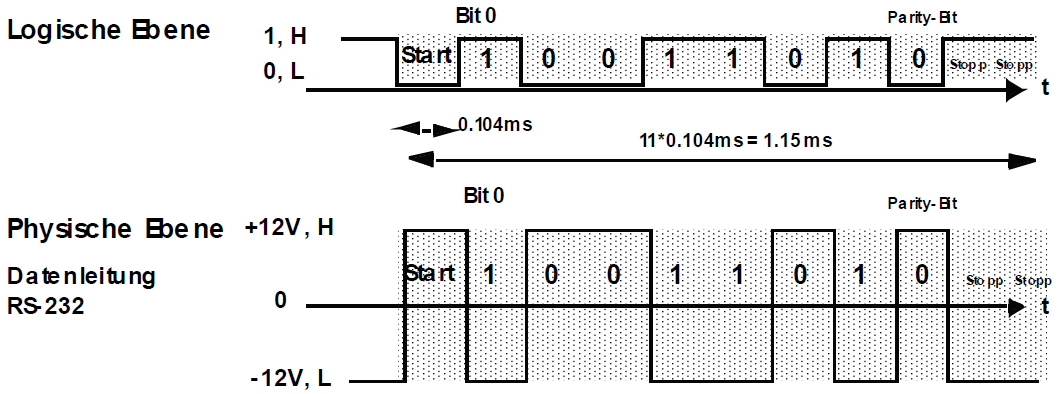
\includegraphics[width= 12cm, height=3cm]{pictures/RS2323_Signalverlauf}
  \begin{itemize}
    \item Das Paritätsbit bewirkt, dass bei gerader („EVEN“) Parität immer eine
    gerade bzw. bei ungerader („ODD“) Parität eine ungerade Anzahl von „1“-Bits übertragen wird. Es gibt also die Möglichkeiten „E“ wie even parity oder „O“ wie odd parity oder kein Parity-Bit entsprechend „N“ wie no parity. Weiterhin kann das Paritätsbit immer gesetzt („M“ wie mark parity) oder immer gelöscht („S“ wie space parity) sein. Abgeschlossen wird die Übertragung mit ein oder zwei Stoppbits logisch „1“
    \item Das LSB wird zuerst geschickt
  \end{itemize}
\subsubsection{Datenleitungen}
\begin{tabular}{|l|l|p{12cm}|}
  \hline
  \textbf{Abkürzung} & \textbf{Name} & \textbf{Beschreibung}\\ \hline
  TxD, TX, TD & Transmit Data & Leitung für ausgehende (von DTE gesendete) Daten
  (negative Logik)\\ 
  \hline
  RxD, RX, RD & Receive Data & Leitung für eingehende (von DTE zu empfangende)
  Daten (negative Logik).\\ 
  \hline
  RTS & Request to Send & „Sendeanforderung“; Ein High-Pegel an diesem Ausgang
  signalisiert, dass DTE Daten senden möchte.\\
  \hline
  CTS & Clear to Send & „Sendeerlaubnis“; Ein High-Pegel an diesem Eingang ist
  ein Signal der Gegenstelle, dass sie Daten von DTE entgegennehmen kann.\\
  \hline
  DSR & Data Set Ready & Ein High-Pegel an diesem Eingang ist ein Signal der
  Gegenstelle, dass sie im Prinzip einsatzbereit ist (aber nicht
  notwendigerweise auch empfangsbereit, siehe CTS)\\
  \hline
  DCD, CD, RLSD & (Data) Carrier Detect & Mit einem High-Pegel an diesem Eingang
  signalisiert die Gegenstelle, dass sie einlaufende Daten auf der Leitung
  erkennt (dem Namen nach ist das die Modulationsträger-Erkennung) und an DTE
  weitergeben möchte.\\
  \hline
  DTR & Data Terminal Ready & Mit einem High-Pegel an diesem Ausgang
  signalisiert DTE seine Betriebsbereitschaft an die Gegenstelle. Damit kann die
  Gegenstelle, z. B. ein Modem, aktiviert oder auch zurückgesetzt werden.
  Üblicherweise antwortet die Gegenstelle mit einem High-Pegel auf DSR.\\
  \hline
  RI & Ring Indicator & Ein High-Pegel an diesem Eingang signalisiert dem
  DTE-Gerät, dass ein Anruf ankommt, d.h. dass jemand eine Datenverbindung
  aufzubauen wünscht, („ring“ ist engl. für „klingeln“; besonders bei Telefonen
  und im übertragenen Sinne auch bei Modems).\\ 
  \hline
  
\end{tabular}

\end{document}
